\documentclass[11pt]{article}

%% FONTS
%% To get the default sans serif font in latex, uncomment following line:
 \renewcommand*\familydefault{\sfdefault}
%%
%% to get Arial font as the sans serif font, uncomment following line:
%% \renewcommand{\sfdefault}{phv} % phv is the Arial font
%%
%% to get Helvetica font as the sans serif font, uncomment following line:
% \usepackage{helvet}
\usepackage[small,bf,up]{caption}
\renewcommand{\captionfont}{\footnotesize}
\usepackage{tikz,pgfplots}
\usepackage[left=1in,right=1in,top=1in,bottom=1in]{geometry}
\usepackage{graphics,epsfig,graphicx,float,subfigure,color}
\usepackage{amsmath,amssymb,amsbsy,amsfonts,amsthm}
\usepackage{url}
\usepackage{boxedminipage}
\usepackage[sf,bf,tiny]{titlesec}
 \usepackage[plainpages=false, colorlinks=true,
   citecolor=blue, filecolor=blue, linkcolor=blue,
   urlcolor=blue]{hyperref}
\usepackage{enumitem}

\newcommand{\todo}[1]{\textcolor{red}{#1}}
% see documentation for titlesec package
% \titleformat{\section}{\large \sffamily \bfseries}
\titlelabel{\thetitle.\,\,\,}

\newcommand{\bs}{\boldsymbol}
\newcommand{\alert}[1]{\textcolor{red}{#1}}
\setlength{\emergencystretch}{20pt}

\begin{document}


\begin{center}
  \vspace*{-2cm}
{\small MATH-GA 2011.002 and CSCI-GA 2945.002, Georg Stadler (NYU Courant)}
\end{center}
\vspace*{.5cm}
\begin{center}
\large \textbf{%%
Fall 2019: Advanced Topics in Numerical Analysis: \\
Finite Element Methods \\
Assignment 2 (due Oct 25, 2019) \\
\\
Terrence Alsup}
\end{center}

% ****************************

\begin{enumerate}
% --------------------------
\item  {\bf Stiffness matrices for $P_1$ and $Q_1$ elements.}
  As shown in Figure~\ref{fig1}, we discretize a square domain with
  either:
  \begin{itemize}
  \item 8 triangles and linear Lagrangian finite elements with nodal basis functions
    corresponding to the corners ($P_1$ elements), or with
  \item  4 quadrilaterals and bilinear Lagrangian elements, also with
    nodal basis functions corresponding to the corners ($Q_1$ elements).
  \end{itemize}
%
\begin{figure}[h!]\centering
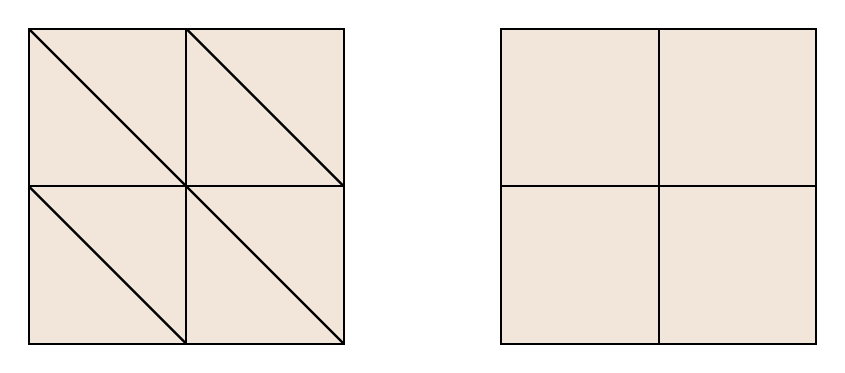
\begin{tikzpicture}
  \foreach \x in {0,2}{
    \foreach \y in {0,2}{
      \filldraw[draw=black,thick,fill=brown!20!white] (\x,\y) rectangle ++(2,2);
      \draw[draw=black,thick] (\x+2,\y) -- (\x,\y+2);
      \draw[draw=black,thick,fill=brown!20!white] (\x+6,\y) rectangle ++(2,2);
    }
  }
\end{tikzpicture}
\caption{Two different discretization of a square using triangles and
  quadrilaterals.\label{fig1}}
\end{figure}
We study the resulting stiffness matrices for the Laplace
equation, neglecting Dirichlet boundary conditions. Each element leads
to a local stiffness matrix $A^k\in \mathbb R^{l\times l}$, with $l\in
\{3,4\}$. You don't need to compute the entries of these matrices
explicitly, but we want to assemble them into the global stiffness
matrix $A^*$.
\begin{enumerate}
  \item Check that for both discretizations, the global number of
    unknowns of solutions is the same, and choose a global numbering.
    Then, perform a matrix assembly in which you simply denote all
    non-zero entries in $A^*$ by $\star$, assuming that all entries in
    the local stiffness matrices are non-zero. This will result in a
    sparsity pattern for the stiffness matrix. These sparsity patterns
    shows which degrees of freedoms are directly couple to each other.\\
\\

%%%%%%%%%%%%%%%%%%%%%%%%%%%%%%%%%%%%%%%%%%%%%%%%%%%%%%%%%%%%%%

{\bf Solution}\\
Both discretizations have $9$ global unknowns corresponding to the $9$ vertices in each.  For a global numbering we will label them from left-to-right and top-to-bottom.  The upper-left node is labeled $1$ and the bottom right node is labeled $9$.  First we look at the global stiffness matrix for the first discretization.  An entry $(i,j)$ will be non-zero when the support of the basis functions $\phi_i$ and $\phi_j$ overlap.  We get that for the discretization with $P_1$
\[
A^{*} = \begin{bmatrix}
* & * &   & * & * &   &   &   &   \\
* & * & * &   & * & * &   &   &   \\
  & * & * &   &   & * &   &   &   \\
* &   &   & * & * &   & * & * &   \\
* & * &   & * & * & * &   & * & * \\
  & * & * &   & * & * &   &   & * \\
  &   &   & * &   &   & * & * &   \\
  &   &   & * & * &   & * & * & * \\
  &   &   &   & * & * &   & * & *
\end{bmatrix}
\]
and similarly for $Q_1$
\[
A^* = \begin{bmatrix}
* & * &   & * & * &   &   &   &   \\
* & * & * & * & * & * &   &   &   \\
  & * & * &   & * & * &   &   &   \\
* & * &   & * & * &   & * & * &   \\
* & * & * & * & * & * & * & * & * \\
  & * & * &   & * & * &   & * & * \\
  &   &   & * & * &   & * & * &   \\
  &   &   & * & * & * & * & * & * \\
  &   &   &   & * & * &   & * & *
\end{bmatrix}
\]



%%%%%%%%%%%%%%%%%%%%%%%%%%%%%%%%%%%%%%%%%%%%%%%%%%%%%%%%%%%%%%%



  \item In FE methods, the sparsity (i.e., large number of zero
    entries compared to non-zero entries) of the finite element
    matrices is important as it allows for fast linear solvers. For
    which method is the global stiffness matrix sparser, and which
    method do you think will be more accurate?\\
\\
%%%%%%%%%%%%%%%%%%%%%%%%%%%%%%%%%%%%%%%%%%%%%%%%%%%%%%%%%%%%%%%

{\bf Solution}\\
The global stiffness matrix is sparser for the triangular discretization simply because there is less overlap between the basis functions.  For instance, the basis function corresponding to the middle vertex will have support that overlaps with all basis functions in the case of quadrilateral elements.  We can also see visually from the matrices $A^*$ that triangular discretization gives a more sparse stiffness matrix.  Moreover, since the triangular discretization is finer with more elements we expect this discretization to give more accurate results.  This is because we can resolve the true function on a finer scale.\\
\\


%%%%%%%%%%%%%%%%%%%%%%%%%%%%%%%%%%%%%%%%%%%%%%%%%%%%%%%%%%%%%%%
  \item Give the stiffness matrices $A$, again using $\star$ for
    non-zero entries, assuming homogeneous Dirichlet boundary for the
    bottom edge of the domain only (for the remainder of the boundary,
    we assume natural, i.e., Neumann boundary conditions, and thus the
    stiffness matrix does not need to be modified for those unknowns.\\
\\
%%%%%%%%%%%%%%%%%%%%%%%%%%%%%%%%%%%%%%%%%%%%%%%%%%%%%%%%%%%%%%%

{\bf Solution}\\
To obtain the stiffness matrices $A$ corresponding to homogeneous Dirichlet boundary conditions along the bottom edge we just need to delete the last 3 rows and columns of $A^*$.  This is due to our choice in labeling the vertices since we labeled the bottom vertices $7,8,9$ last.  Thus, for the discretization with $P_1$ we get
\[
A = \begin{bmatrix}
* & * &   & * & * &    \\
* & * & * &   & * & *   \\
  & * & * &   &   & *    \\
* &   &   & * & * &      \\
* & * &   & * & * & *\\
  & * & * &   & * & * 
\end{bmatrix}
\]
and similarly for $Q_1$
\[
A = \begin{bmatrix}
* & * &   & * & * &      \\
* & * & * & * & * & *    \\
  & * & * &   & * & *   \\
* & * &   & * & * &      \\
* & * & * & * & * & *  \\
  & * & * &   & * & * 
\end{bmatrix}
\]

%%%%%%%%%%%%%%%%%%%%%%%%%%%%%%%%%%%%%%%%%%%%%%%%%%%%%%%%%%%%%%%
\end{enumerate}



\item {\bf A 1D Hermite element.}  Consider the finite element
  $(K,\mathcal P,\mathcal N)$ with $K=(0,1)$, $\mathcal P=P_3$, the
  space of cubic polynomials, and $\mathcal N=\{N_1,\ldots,N_4\}$
  defined as $N_1(v)=v(0)$, $N_2(v)=v'(0)$, $N_3(v)=v(1)$,
  $N_4(v)=v'(1)$.
  \begin{enumerate}
  \item Show that $\mathcal N$ determines $\mathcal P$.\\
\\
%%%%%%%%%%%%%%%%%%%%%%%%%%%%%%%%%%%%%%%%%%%%%%%%%%%%%%%%%%%%%%%

{\bf Solution}

Suppose that $v \in \mathcal P$ is a cubic polynomial $v(x) = ax^3 + bx^2 + cx + d$ and that $N_i(v) = 0$ for $i=1,2,3,4$.  We are to show that $v \equiv 0$.  We have that $N_1(v) = v(0) = d = 0$.  We also have $N_2(v) = v'(0) = c = 0$.  The last two equations are $N_3(v) = v(1) = a + b = 0$ and $N_4(v) = v'(1) = 3a + 2b = 0$.  In matrix form we have
\[
\begin{bmatrix}
1 & 1\\
3 & 2
\end{bmatrix}\begin{bmatrix}
a\\
b
\end{bmatrix} = \begin{bmatrix}
0\\
0
\end{bmatrix}
\]
Since the determinant of this matrix is non-zero we know that the only solution is $a = b = 0$.  Hence $v \equiv 0$ and $\mathcal N$ determines $\mathcal P$.



%%%%%%%%%%%%%%%%%%%%%%%%%%%%%%%%%%%%%%%%%%%%%%%%%%%%%%%%%%%%%%%
  \item Construct the nodal basis, i.e., the dual basis for this
    finite element in terms of the monomial basis
    $\{1,x,x^2,x^3\}$.\\
\\
%%%%%%%%%%%%%%%%%%%%%%%%%%%%%%%%%%%%%%%%%%%%%%%%%%%%%%%%%%%%%%%

{\bf Solution}\\
The dual basis is the basis $\phi_{j}$ for $j=1,2,3,4$ such that $N_i(\phi_j) = \delta_{ij}$.  If we write
\[
\phi_j(x) = a_jx^3 + b_jx^2 + c_jx + d_j
\]
then the conditions that $N_i(\phi_j)$ for $i,j = 1,2,3,4$ gives a linear system of 16 equations in the variables $\{a_j,b_j,c_j,d_j\}_{j=1}^4$ (similar to a Vandermonde matrix).  We have that
\begin{align*}
N_1(\phi_j) &= \phi_j(0) = d_j = \delta_{1j}\\
N_2(\phi_j) &= \phi_j'(0) = c_j = \delta_{2j}\\
N_3(\phi_j) &= \phi_j(1) = a_j + b_j + c_j + d_j = \delta_{3j}\\
N_4(\phi_j) &= \phi_j'(1) = 3a_j + 2b_j + c_j = \delta_{4j}
\end{align*}
Solving this system of equations gives the dual basis
\begin{align*}
\phi_1(x) &= 2x^3 - 3x^2 + 1\\
\phi_2(x) &= x^3 - 2x^2 + x\\
\phi_3(x) &= -2x^3  +3x^2\\
\phi_4(x) &= x^3 - x^2 
\end{align*}


%%%%%%%%%%%%%%%%%%%%%%%%%%%%%%%%%%%%%%%%%%%%%%%%%%%%%%%%%%%%%%%
  \end{enumerate}
 Consider the problem
 \begin{equation}
   -u'' + u = f, \quad u'(0) = 0,\: u'(1)=0.
 \end{equation}
 Discretize the domain $\Omega=(0,1)$ into $N$ intervals of uniform
 mesh size $h=1/N$ and let $V_h$ be the space constructed by
 equipping each cell with the Hermite finite element defined
 above. This induces a linear system $AU=F$.
 \begin{enumerate}

 \setcounter{enumii}{2}
 \item State the abstract expressions for the stiffness matrix $A$
   and the load vector $F$.\\
\\
%%%%%%%%%%%%%%%%%%%%%%%%%%%%%%%%%%%%%%%%%%%%%%%%%%%%%%%%%%

{\bf Solution}\\
We first obtain the weak form by multiplying by a test function $v \in H_0^1((0,1))$.
\[
\int_0^1 -u''v + uv\ dx = \int_0^1 fv\ dx
\]
Integrating by parts gives
\[
a(u,v) := \int_0^1 u'v' + uv\ dx = \int_0^1 fv\ dx =: \ell(v)
\]
Note that the boundary terms vanished because we assume that $u'(0) = u'(1) = 0$.  Since we have partitioned the interval into $N$ intervals we have a total of $N + 1$ vertices.  Each vertex requires the function and derivative value so we will need $2(N+1)$ basis functions.  However, the derivatives at the endpoints are fixed by our boundary conditions we only actually need $2N$ global basis functions $\Phi_i$.  The entries of the global stiffness matrix and load vector are given abstractly by
\[
A_{ij} = a(\Phi_i,\Phi_j)\quad F_{i} = \ell(\Phi_i),\quad \text{ for }\quad i,j = 1,\ldots,2N
\]
Here we'll use the convention that
\[
\Phi_{2k+1}(x) = \begin{cases}
\phi_3\left( N(x - (k-1)/N) \right) & x \in [(k-1)/N,\ k/N]\\
\phi_1\left( N(x - k/N) \right) & x \in [k/N, (k+1)/N]\\
0 & \text{ otherwise}
\end{cases}
\]
for $k=0,\ldots,N$ which corresponds to the function evaluation at the $N+1$ vertices in the mesh.  Similarly, we define
\[
\Phi_{2k}(x) = \begin{cases}
\phi_4 \left( N(x - (k-1)/N) \right) & x \in [(k-1)/N,\ k/N]\\
\phi_2\left( N(x - k/N) \right) & x\in [k/N,\ (k+1)/N]\\
0 & \text{ otherwise}
\end{cases}
\]
for $k=1,\ldots,N+1$ which corresponds to the derivative evaluation at the $N-1$ interior nodes. Setting the coefficients for the basis functions $\Phi_2,\Phi_{2(N+1)}$ to $0$ gives the $2N$ degrees of freedom.\\
\\

%%%%%%%%%%%%%%%%%%%%%%%%%%%%%%%%%%%%%%%%%%%%%%%%%%%%%%%%%%
 \item For one cell $K$, give the local stiffness matrix $A^k\in
   \mathbb R^{4\times 4}$.\\
\\
%%%%%%%%%%%%%%%%%%%%%%%%%%%%%%%%%%%%%%%%%%%%%%%%%%%%%%%%%%

{\bf Solution}\\
If we let cell $K$ be $[(k-1)/N,\ k/N]$ for $k=1,\ldots,N$, then we write the elements of the local stiffness matrix $A^k$ using
\begin{align*}
A^k_{ij} &  \\
=& \int_{(k-1)/N}^{k/N} \left\{N^2\phi_i'(Nx - (k-1))\phi_j'(Nx - (k-1)) + \phi_i(Nx - (k-1))\phi_j(Nx - (k-1)) \right\} \ dx
\end{align*}
for $i,j = 1,2,3,4$.  Using the change of variables $\xi = Nx - (k-1)$ we get
\[
A^k_{ij} = \int_0^1 \left\{N\phi_i'(\xi)\phi_j'(\xi) + N^{-1}\phi_i(\xi)\phi_j(\xi) \right\} \ d\xi
\]
Using Mathematica to compute the integrals we obtain
\[
A^k = N \begin{bmatrix}
6/5 & 1/10 & -6/5 & 1/10\\
1/10 & 2/15 & -1/10 & -1/30 \\
-6/5 & -1/10 & 6/5 & -1/10\\
1/10 & -1/30 & -1/10 & 2/15
\end{bmatrix}+ N^{-1}\begin{bmatrix}
13/35 & 11/210 & 9/70 & -13/420 \\
11/210 & 1/105 & 13/420 & -1/140 \\
9/70 & 13/420 & 13/35 & -11/210 \\
-13/420 & -1/140 & -11/210 & 1/105
\end{bmatrix}
\]
for every cell $K = 1,\ldots,N$.\\
\\

%%%%%%%%%%%%%%%%%%%%%%%%%%%%%%%%%%%%%%%%%%%%%%%%%%%%%%%%%%
 \item Use the finite element matrix assembly algorithm to construct
   the matrix A for the case $N=3$.\\
\\
%%%%%%%%%%%%%%%%%%%%%%%%%%%%%%%%%%%%%%%%%%%%%%%%%%%%%%%%%%

{\bf Solution}\\
We first assemble the matrix $A^*$ which ignores boundary conditions.  We have that $A^*_{ij} = a(\Phi_i, \Phi_j)$ for $i,j = 1,\ldots,2(N+1)$.  To assemble the global stiffness matrix we use the connectivity array $M$ which is the $N \times 4$ matrix given below.
\[
M = \begin{bmatrix}
1 & 2 & 3 & 4\\
3 & 4 & 5 & 6\\
5 & 6 & 7 & 8
\end{bmatrix}
\]
To compute the global stiffness matrix $A^*$ from the connectivity array $M$ and the local stiffness matrices we add $A^k_{ij}$ to $A^*$ at the index $(M_{ki}, M_{kj})$ for all $i,j = 1,2,3,4$ and $k = 1,2,3$.    The result is the desired $8\times 8$ matrix.  To obtain the global stiffness matrix $A$ that takes the homogeneous Neumann conditions into account, we simply delete rows and columns $2$ and $2N + 1 = 7$ from $A^*$, which corresponded to the basis functions at the ends of the interval with zero derivatives.  The final result is a $6\times 6$ matrix.\\
\\

%%%%%%%%%%%%%%%%%%%%%%%%%%%%%%%%%%%%%%%%%%%%%%%%%%%%%%%%%%
 \end{enumerate}
 %*********************

\item {\bf Numerical quadrature for local stiffness matrices.} As
  discussed in class, in most cases it is not possible to analytically
  compute the integrals in the computation of the stiffness matrix
  elements. Thus, one usually has to resort to numerical quadrature. A quadrature
  on an element $K$ has degree of precision $m$ if it computes the
  exact result for all polynomials of degree $m$ or less.
  We consider two cases:
  \begin{itemize}
  \item Quadratic Lagrange elements and constant coordinate
    transformation Jacobian, for the bilinear form
    \begin{equation}\label{eq:K}
      a(u,v) = \int_\Omega\nabla u \cdot \nabla v\,dx,
    \end{equation}
  \item Fourth-order Lagrange elements and linear coordinate
    transformation Jacobian, for the bilinear form
    \begin{equation}\label{eqLM}
      a(u,v) = \int_\Omega u v\,dx.
    \end{equation}
  \end{itemize}
  \begin{enumerate}
  \item What is the minimum degree of precision required to exactly
    assemble the matrices for these bilinear forms?\\
\\
%%%%%%%%%%%%%%%%%%%%%%%%%%%%%%%%%%%%%%%%%%%%%%%%%%%%%

{\bf Solution}\\
If the basis functions $\phi_i$ are quadratic polynomials, the gradients $\nabla \phi_i$ will be linear polynomials and the product $\nabla \phi_i \cdot \nabla \phi_j$ will be a polynomial of degree at most $2$.  Thus, to assemble the local stiffness matrices exactly we will need a minimum degree of precision of $m = 2$.\\
\\
If the basis functions $\phi_i$ are fourth-order polynomials, then the products $\phi_i\phi_j$ will be polynomials of degree at most $8$.  Thus, the minimum degree of precision is $m = 8$.

%%%%%%%%%%%%%%%%%%%%%%%%%%%%%%%%%%%%%%%%%%%%%%%%%%%%%
  \item In one dimension, how many quadrature points are required for
    exact results when using Gaussian quadrature?\\
\\
%%%%%%%%%%%%%%%%%%%%%%%%%%%%%%%%%%%%%%%%%%%%%%%%%%%%%

{\bf Solution}\\
For Gaussian quadrature in 1D with $n$ points we can integrate polynomials of degree at most $2n-1$ exactly.  Thus for the first bilinear form with quadratic elements we will need at least $n = 2$ quadrature points, and for the second bilinear form with fourth-order Lagrange elements we will need at least $n = 5$ points.


%%%%%%%%%%%%%%%%%%%%%%%%%%%%%%%%%%%%%%%%%%%%%%%%%%%%%
  \end{enumerate}

\end{enumerate}




\end{document}
